\documentclass[../main.tex]{subfiles}

\begin{document}

\section{Related Works}
\label{sec: Related Works}

\subsection{Inflation Forecasts}
\label{sub: Inflation Forecasts}

Accurate forecasts of future inflation is important for policymakers conducting monetary and fiscal policy.
Inflation is also significant when investors hedge the risk of nominal assets; when companies make investment decisions or determine the prices; and when labor and management negotiate wages.

Short-term forecasts of inflation is difficult, so various methods have been devised.
This section introduces the study of Ang et al., which comprehensively compares econometric methods, and describes \emph{artificial neural networks (ANN)}.

\subsubsection{Comparison of econometric methods and surveys}

Ang et al.~\cite{Ang2007} applied four methods to U.S. inflation forecasts and compared their forecasting accuracy.  They used time-series models, regressions using real activity measures motivated from the Phillips curve, term structure models that include linear and non-linear specifications, and survey-based measures.
As a result, the surveys were the most accurate.
Additionally they examined combining methods.  However, the combinations of these forecasting methods were not able to achieve higher accuracy than the survey alone.

The forecasting methods they used are roughly four, but each method has several variations depending on the parameters of time-series models, economic indicators included in the regressions or term structure models, and the aggregating methods of forecasting values collected by surveys.
They also used three surveys: the Livingston Survey (LIV), the Survey of Professional Forecasters (SPF), and the Michigan survey (MICH).
We describe the Livingston Survey and the SPF in Section~\ref{ssub: Surveys}.

The target of forecasts are annual change rates of four inflation indicators: Consumer Price Index for All Urban Consumers, All Items (CPI); CPI for All Urban Consumers, All Items Less Shelter (CPI-XS); CPI for All Urban Consumers, All Items Less Food and Energy (CoreCPI); and Personal Consumption Expenditure (PCE).
Ang et al.\ set two out-of-sample periods, after 1985 and 1995.
And they evaluated the forecasting methods by Root Mean Squared Errors (RMSE) during that periods.

\begin{table}
  \caption{
    Empirical results by Ang et al.~\cite{Ang2007}.
    Each entry represents the ratio of the RMSE to a benchmark, ARMA(1,1).
    Bold entries are the smallest RMSEs in each column.
    The rows represents forecasting methods: the best time-series model (not necessarily ARMA(1,1)), the best Phillips Curve models, the best term structure model, and three surveys, LIV, SPF and MICH\@.  The bottom row is the ensemble method by weighted averaging all models.
    Each method is applied to two out-of-sample periods, post-1985 and post-1995.
  }\label{tab: ang}
  \begin{center}
    \begin{tabular}{llrrrr}
\toprule
          &             &    CPI &  CPI-XS &  CoreCPI &    PCE \\
\midrule
Post-1985 & Time-Series &  1.000 &   1.000 &     1.000 &  1.000 \\
          & Phillips-Curve &  0.979 &   1.000 &     0.862 &  1.027 \\
          & Term-Structure &  1.091 &   1.047 &     0.945 &  1.018 \\
          & LIV &  0.789 &   0.844 &\textbf{0.655}&  1.082 \\
          & SPF &\textbf{0.779}&\textbf{0.819}&     0.691 &  1.199 \\
          & MICH &  0.902 &   0.881 &     1.185 &  1.217 \\
          & Ensemble &  0.873 &   0.864 &     0.819 &\textbf{0.962}\\ \midrule
Post-1995 & Time-Series &  0.764 &   0.833 &     0.915 &\textbf{1.000}\\
          & Phillips-Curve &  0.977 &   0.992 &     0.767 &  1.020 \\
          & Term-Structure &  0.913 &   0.973 &     0.866 &  1.025 \\
          & LIV &  0.792 &   0.856 &     0.557 &  1.202 \\
          & SPF &  0.861 &   0.914 &\textbf{0.699}&  1.250 \\
          & MICH &  0.862 &   0.937 &     0.822 &  1.338 \\
          & Ensemble &\textbf{0.722}&\textbf{0.735}&     0.702 &  1.005 \\
\bottomrule
\end{tabular}

  \end{center}
\end{table}

Table~\ref{tab: ang} shows the empirical results by Ang et al.
Each value reports the relative RMSE ratio to a time-series model, ARMA(1,1).
In time-series models, ARMA(1,1) generally showed good accuracy, so it was set as the benchmark.
The Phillips Curve models and the term structure models were sometimes worse than the benchmark and they never achieve the best score in each column.
Overall, the surveys outperformed the other forecasting methods.

Ang et al.\ investigated ensemble methods such as mean, median and weighted average.
Weighted average made the most accurate forecasts among them.  The table shows the RMSEs of the weighted average as an ensemble method.
The ensemble method had the smallest RMSEs in only three of the eight.  Combining forecasts did not always make more accurate forecasts.

\subsubsection{Artificial neural networks}

Inflation forecasting using an ANN model has been studied recently\cite{Choudhary2012, Moshiri2000, Nakamura2005}.
These studies have reported that ANN models can forecast as well as traditional time-series models and sometimes outperform them.
This section describes ANN models.

ANN is a method of machine learning that is inspired biological learning system~\cite{Mitchell1997}.  It has attracted much attention with the development of deep learning~\cite{岡谷2015}.

\begin{figure}
  \centering
  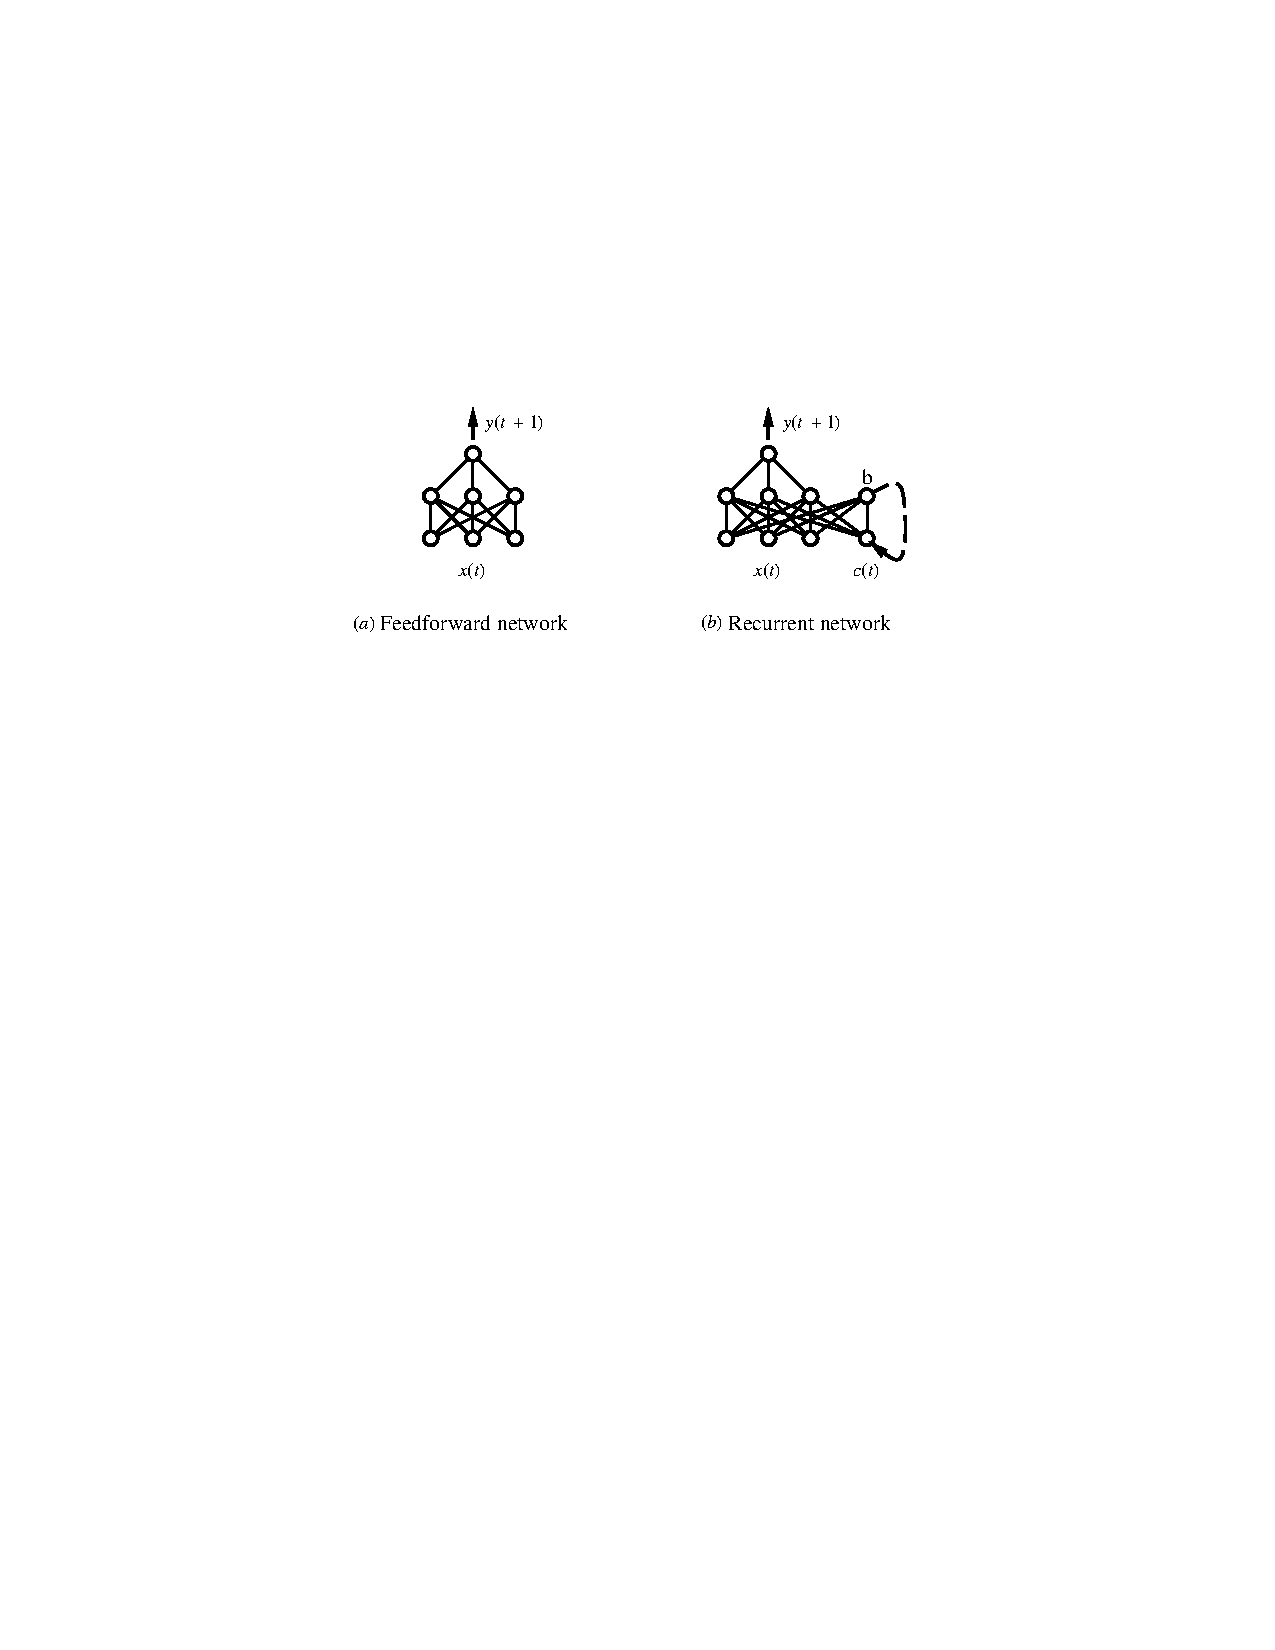
\includegraphics[width=0.8\textwidth]{related-rnn.pdf}
  \caption{
    Architecture of a feedforward network and recurrent network~\cite{Mitchell1997}.
  }\label{fig: RNN}
\end{figure}

Figure~\ref{fig: RNN} (a) shows the basic architecture of an ANN\@.  An ANN consists of layers that include some units called \emph{neuron}.
A unit $i$ receives an input vector $\x_i$ and returns an output $o_i(\x)$.
The output $o_i(\x)$ is
\begin{equation}
  o_i(\x_i) = f(\bm{w}_i \cdot \x_i + b_i),
\end{equation}
where $\bm{w_i}$ is weights, $b_i$ is a bias, and $f$ is an \emph{activation function}.
Each unit multiplies the inputs by the weights, adds a bias, and returns the output of the activation function with it.
The logistic function or rectified linear function is used for activation functions.
And an activation function suitable for the problem is used as the output layer of the network.
In a feedforward network, a unit receives the outputs of units in the previous layer and its output is received by units in the next layer.  By repeating this, the network can express non-linear function $y(\x)$.
For example, it is possible to create a classifier that estimates the age and sex from a face photo.

An ANN learns by adjusting the weights $\bm{w}$ and biases $b$ so as to approach the input and output of the training set.
Regard parameters $\bm{w}$ include weights and biases.
The training set consists of pairs of inputs $\x$ and target outputs $\bm{d}$, $\{(\x_1,\bm{d}_1), (\x_2,\bm{d}_2), \dots, (\x_N,\bm{d}_N)\}$.
The \emph{Gradient Descent} is used for the parameter adjustment.
It updates the parameters $\bm{w}$ gradually so as to reduce the error function $E(\bm{w})$, which represents the error between the output of the network $y$ and target output $\bm{d}$.  That is,
\begin{equation}
  \bm{w} \gets \bm{w} - \eta \nabla E,
\end{equation}
where $\eta$ is a learning rate and $\nabla E$ is a gradient defined as
\begin{equation}
  \nabla E \equiv \left[\frac{\partial E}{\partial w_{0}},
\frac{\partial E}{\partial w_{1}}, \cdots \frac{\partial E}{\partial
w_{n}}\right].
\end{equation}
The \emph{Stochastic Gradient Descent}, which updates parameters using not all samples but a batch of a plurality of samples, is often used.
It has been proved that learning converges if learning rate is sufficiently small.
For efficient gradient calculation, the \emph{Backpropagation} algorithm is generally used.

\emph{Recurrent neural networks (RNN)} are neural networks including circular structures as shown in Figure~\ref{fig: RNN} (b), and are applied to time series data.
For example, A RNN model can predict the stock price of the next day based on the fluctuations of the price so far.
Learning of RNN also uses the Gradient Descent, and the learning algorithm is the extended Backpropagation.

\subsection{Wisdom of the Crowd}
\label{sub: Wisdom of the Crowd}

A journalist Surowiecki~\cite{Surowiecki2004} has summarized phenomena where groups of humans made more accurate forecast than an expert.  He called it the \emph{wisdom of the crowd}.
The reason why the wisdom of the crowd works well is that individuals in the group have diverse information.
For instance, while several people forecast that the GDP will increase due to a policy, others forecast that it will decrease due to recession in a country, so the aggregation of them can make more informative forecasts.
The results of Ang et al., where the surveys outperform various forecasting methods, can be explained by the wisdom of the crowd.

Page~\cite{Page2008} gave the a rationale for the wisdom of the crowd.
\emph{Diversity prediction theorem} states ``a crowd's collective accuracy equals the average individual accuracy minus their collective predictive diversity.''
Let $h_i$ denote forecasted value by individual $i$, and let $\bar{h}$ denote the average of $N$ forecasts.  $V$ is a correct value.
Then, the following equation always holds~\cite{Krogh1995, Page2008}.
\begin{equation}
  {(V - \bar{h})}^2 = \frac{1}{N}\sum_{i=1}^N {(V - h_i)}^2 - \frac{1}{N}\sum_{i=1}^N {(\bar{h} - h_i)}^2
\end{equation}

The left side is the squared error of the group's forecast $\bar{h}$.
The first term on the right side is the average of the squared error of each individual forecast.
The second term is the variance of the forecasts within the group, which represents the diversity of the forecasts within the group.
This value decreases as the individuals in the group make similar forecasts, and increases as they make diverse forecasts.
The larger this values, the smaller the error of the group forecast (the left side) compared with the forecast error of average individual (the first term on the right side).
This is because the averaging the forecasts with positive error and ones with negative error offset the errors.

\subsection{Ensemble Methods}
\label{sub: Ensemble Methods}

This section describes \emph{weighted averaging} and a study on the optimal composition of a group in the case where individual forecasters have types such as professional and non-professional.

In weighted averaging, the optimal weights can be obtained when given a covariance matrix of forecasters' errors~\cite{Zhou2012}.
Let $h_i$ denote a forecasted value by a forecaster $i$, and let $w_i$ denote $i$'s weight.
When a vector of forecasts by $N$ forecasters $\bm{h} = (h_1, \ldots, h_N)$ is given, the weighted average $G(\bm{h})$ is
\begin{equation}
  G(\bm{h}) = \sum_{i=1}^N w_i \cdot h_i,
  \label{eq: weighted average}
\end{equation}
where $w_i \geq 0$ and $\sum_i w_i = 1$.
The weights $\bm{w} = (w_1, \ldots, w_N)$ are determined to minimize $G$'s expected squared error $\MSE(G)$:
\begin{equation}
  \bm{w} = \argmin_{\bm{w}} \MSE(G).
\end{equation}

Let $\cov(\varepsilon_{h_i},\varepsilon_{h_j})$ denote the covariance in the errors of the forecasters $i$ and $j$, and let $\var(\varepsilon_{h_i}) (= \cov(\varepsilon_{h_i},\varepsilon_{h_i}))$ denote the variance of forecaster $i$.  Then $w_i$ that minimizes the expected squared error is obtained by
\begin{equation}
  w_i = \frac
      {\sum_{j=1}^N {\cov(\varepsilon_{h_i}, \varepsilon_{h_j})}^{-1}}
      {\sum_{k=1}^N \sum_{j=1}^N {\cov(\varepsilon_{h_k}, \varepsilon_{h_j})}^{-1}}.
\end{equation}
The covariance matrix can be estimated from past forecasts.
Basically, weighted averaging gives big weights to accurate forecasters, and small ones to inaccurate forecasters.
However, if the covariance is small, that is, forecasters make errors differently from each other, the weights of those are set not to be too biased to either one.

Weighted averaging assumes that the number of forecasters $N$ is constant.
And it cannot make use of the good points of each forecaster as mentioned in \ref{sec: Introduction} since the weights $\bm{w}$ are fixed regardless of the input $\x$.
In other words, even if forecaster $i$ can make an accurate forecast for input $\x_1$ but can not do so for input $\x_2$, the weights are always same.

Lamberson and Page~\cite{Lamberson2012} proposed to use a ratio of forecaster types instead of weights when the forecasters have types.
The forecasters are divided into types by a statistical criterion called \emph{type coherence}.
Here we assume there are two types of forecasters.
If the number of forecasters is small, the ratio of a type having high accuracy should be increased, and if the number of forecasters is big, the ratio of a type having high diversity should be increased.

There are two types of forecasters, $a$ and $b$.  The number of each is $A$ and $B$ respectively, and the sum is $N = A + B$.
The forecast values of each forecaster is modeled as random variables, and follows a probability distribution according to the type of the forecaster.
Assume that the forecasters are unbiased, that is, forecasts are not always greater or smaller than the real value.
Let $\var(\varepsilon_a)$ and $\var(\varepsilon_b)$ denote the variance of the type $a$ and $b$ respectively.
The variance equals the expected squared error if forecasts are unbiased.
Let $\cov(\varepsilon_a)$ denote the covariance in the errors of the forecasts made by two different type $a$ forecasters, and assume that this is the same for any pair of type $a$ forecasters.  Define $\cov(\varepsilon_b)$ similarly.
The smaller the within-type covariance, the more diverse the group of forecasters.
Finally, let $\cov(\varepsilon_a,\varepsilon_b)$ denote the covariance in the errors of any two forecasters, one of which is of type $a$ and the other of which is of type $b$.
Let us find the ratio of the number of each type $A$ and $B$ that minimizes the expected squared error of the ensemble.

Type coherence between two types $a$ and $b$ is defined as
\begin{equation}
  \TC(a, b) = \cov(\varepsilon_a) + \cov(\varepsilon_b) - 2\cov(\varepsilon_a, \varepsilon_b).
\end{equation}
If $\TC(a, b) > 0$, type $a$ and $b$ satisfy type coherence.
This means the across-type covariance is less than the average of the within-type covariances.

The forecasts of an ensemble is simple averaging.
Then, the expected squared error of the ensemble is
\begin{equation}
  \frac{A\var(\varepsilon_a) + B\var(\varepsilon_b) + 2\binom{A}{2}\cov(\varepsilon_a) + 2\binom{B}{2}\cov(\varepsilon_b) + 2AB\cov(\varepsilon_a,\varepsilon_b)}{N^2}.
  \label{eq: lamberson}
\end{equation}

Given the size of the group $N$, the optimal fraction of type $a$ forecasters, which minimizes that expected squared error, is approximated by
\begin{equation}
  A^\ast = \frac{[\var(\varepsilon_b) - \var(\varepsilon_a)] - [\cov(\varepsilon_b) - \cov(\varepsilon_a)]}{2N \cdot \TC(a, b)} + \frac{\cov(\varepsilon_b) - \cov(\varepsilon_a, \varepsilon_b)}{\TC(a, b)},
  \label{eq: optimal A}
\end{equation}
where the approximation error is less than $1/M^2$.

Focusing on $\var(\varepsilon_a)$ and $\var(\varepsilon_b)$, decreasing $\var(\varepsilon_a)$ or increasing $\var(\varepsilon_b)$ make $A^\ast$ greater.
The more accurate the forecasts of type $a$ or the less accurate the ones of type $b$, the greater the optimal ratio of type $a$ forecasters in the group.

However, if the group size $N$ is sufficiently large, the first term in equation (\ref{eq: optimal A}) can be ignored.
Then, the optimal number of type $a$ forecasters, $A^\ast$ is independent from $\var(\varepsilon_a)$ and $\var(\varepsilon_b)$, and depends on the diversity of each type, not the forecast accuracy of each type.

Lamberson and Page have summaried the above results as follows:
\begin{quote}
  In a sufficiently small group, the lowest variance type should be in the majority.
  In a sufficiently large group, the forecaster type with the lowest within-type covariance should be in the majority~\cite{Lamberson2012}.
\end{quote}
For example, consider conducting economic forecasts by employing a group of forecasters.
If you want reduce the group size, it is better to increase the ratio of forecasters with high capability such as experts, and otherwise, it is better to increase the ratio of ordinary people.

However, the model of Lamberson and Page also can not utilize the characteristics that each type of forecasters has.
For instance, assume that there are two types of forecasters. Type $c$ forecasters use time-series models for economic forecasts, so their forecasts are accurate when the economy is stable; and type $d$ forecasters make forecasts based on economic information, so they can make flexible forecasts even when the economy is unstable.
As well as weighted averaging, the method of Lamberson and Page can not change the combination according to the situation.
The next chapter proposes a human-machine ensemble method that harnesses each advantege, assuming a prediction model obtained by machine learning as type $c$ and humans as type $d$.
\end{document}
